\documentclass{article}
\usepackage[utf8]{inputenc}
\usepackage{amsmath}
\usepackage{tikz}
\usepackage{tikzsymbols}
\usepackage[margin=1in]{geometry}

\title{Chapter 8 Homework}
\author{Damien Koon}
\date{10/28/2022}

\begin{document}

\maketitle

\vspace{2cm}

\begin{center}
    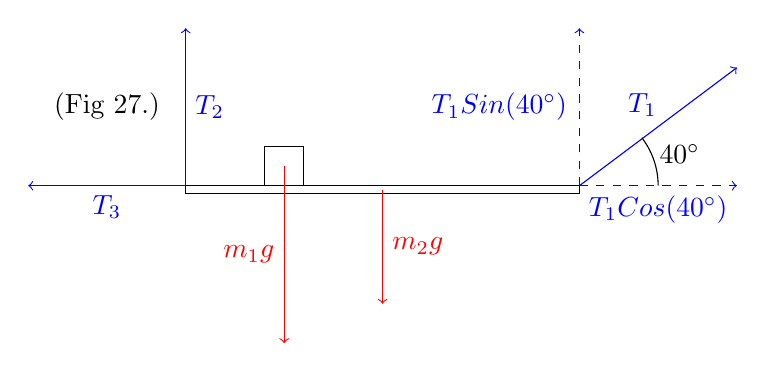
\begin{tikzpicture}
        \draw (0,4.9) rectangle (5,5);
        \draw node at (-1,6) {(Fig 27.)};
        \draw[blue] [->] (0,5) -- node[below] {$T_3$}(-2,5);
        \draw[blue] [->] (0,5) -- node[right] {$T_2$}(0,7);
        \draw[blue] [->] (5,5) -- node[above, xshift=-.2cm] {$T_1$}(7,6.5);
        \draw[dashed, blue] [->] (5,5) -- node[right, xshift=-2cm] {$T_1Sin(40^\circ)$}(5,7);
        \draw[dashed, blue] [->] (5,5) -- node[below] {$T_1Cos(40^\circ)$}(7,5);
        \draw(6,5) arc (0:37.5:1cm and 1cm) node[right, xshift=0.1cm, yshift=-0.2cm] {$40^\circ$};
        \draw (1,5) rectangle (1.5,5.5);
        \draw[red] [->] (1.25,5.25) -- node [left] {$m_1g$}(1.25,3);
        \draw[red] [->] (2.5,4.95) -- node [right] {$m_2g$}(2.5,3.5);
    \end{tikzpicture}
\end{center}

\section {27. A uniform plank of length $2.00 m$ and mass $30.0 kg$ is supported by three ropes. Find the tension in each rope when a $700 N$ person is $0.500 m$ from the left end.}

\begin{trivlist}
\item $$2 T_1 Sin(40) + (0)T_2 = (0.5)(700) + (30)(9.81) \Rightarrow T_1 = \frac{0.5 * 700 + (30)(9.81)}{2Sin(40)} = \underline{501 N} $$

\item $$ T_1\perp + T_2\perp = m_1 g + m_2 g \Rightarrow T_2 = m_1 g + m_2 g - T_1 Sin(40) = (30)(9.81) + 700 - (501 Sin(40)) = \underline{672 N} $$

\item $$T_3 \parallel  = T_1 \parallel  = 501N Cos(40) = \underline{384 N}$$
\end{trivlist}

\begin{center}
    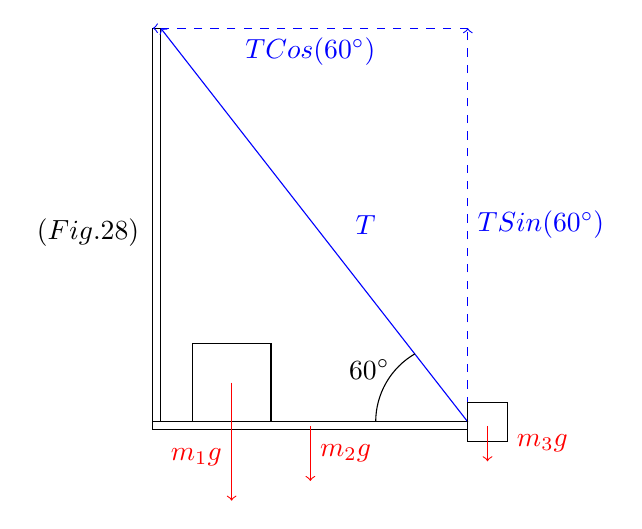
\begin{tikzpicture}
        \draw(0,4.9) rectangle (4,5);
        \draw(0,5) rectangle node[left,xshift=-0.1cm,yshift=-0.1cm] {$(Fig. 28)$} (0.1,10);
        \draw[blue] [->] (4,5) -- node[right, xshift=0.4cm]{$T$}(0.1,10);
        \draw[dashed,blue] [->] (4,5) -- node[right]{$TSin(60^\circ)$} (4,10);
        \draw[dashed,blue] [->] (4,10) -- node[below]{$TCos(60^\circ)$} (0,10);
        \draw(2.83,5) arc (180:120:1cm and 1cm) node[left, xshift=-0.2cm, yshift=-0.2cm] {$60^\circ$};
        \draw(0.5,5) rectangle (1.5,6);
        \draw[red] [->] (1,5.5) -- node[left, yshift=-0.2cm] {$m_1g$}(1,4);
        \draw(4,4.75) rectangle (4.5,5.25);
        \draw[red] [->] (2,4.95) -- node[right]{$m_2g$}(2,4.25);
        \draw[red] [->] (4.25,4.95) -- node[right,xshift=0.25cm]{$m_3g$}(4.25,4.5);
    \end{tikzpicture}
\end{center}


\section {28. A hungry bear weighing $700 N$ walks out on a beam in an attempt to retrieve a basket of goodies hanging at the end of the beam. The beam is uniform, weighs $200 N$, is $6 m$ long, and it is supported by a wire at an angle of $60^\circ$ The basket weighs $80 N$}

\begin{itemize}
    \item a. Draw a force diagram for the beam.
    \item b. When the bear is at $1 m$, find the tension in the wire supporting the beam and the components of the force exerted by the wall on the left end of the beam.
    \item c. If the wire can withstand a maximum tension of
    $900 N$, what is the maximum distance the bear can walk before the wire breaks?
\end{itemize}

\begin{trivlist}

    \item $$r_T T\perp = r_1 m_1 g + r_2 m_2 g + r_3 m_3 g \Rightarrow r_T T Sin(60) = (700N)(1m) + (3m)(200N) + (6m)(80N)$$
    \item $$(6m)(T)(Sin60) = 1780N \Rightarrow T = \frac{1780N}{(6m)(Sin60)} = \underline{343N}$$
    
    \item $$r_T T \perp = r_1 m_1 g + r_2 m_2 g + r_3 m_3 g \Rightarrow r_1 m_1 g = r_T T\perp - r_2 m_2 g - r_3 m_3 g$$
    \item $$r_1 = \frac{(r_T T\perp)-(r_2 m_2 g)-(r_3 m_3 g)}{m_1 g} = \frac{(6m * \textbf{900N} Sin(60)) - (3m * 200N) - (6m * 80N)}{700N} = \underline{5.14 m}$$
    \end{trivlist}

\end{document}
